\documentclass[1p]{elsarticle_modified}
%\bibliographystyle{elsarticle-num}

%\usepackage[colorlinks]{hyperref}
%\usepackage{abbrmath_seonhwa} %\Abb, \Ascr, \Acal ,\Abf, \Afrak
\usepackage{amsfonts}
\usepackage{amssymb}
\usepackage{amsmath}
\usepackage{amsthm}
\usepackage{scalefnt}
\usepackage{amsbsy}
\usepackage{kotex}
\usepackage{caption}
\usepackage{subfig}
\usepackage{color}
\usepackage{graphicx}
\usepackage{xcolor} %% white, black, red, green, blue, cyan, magenta, yellow
\usepackage{float}
\usepackage{setspace}
\usepackage{hyperref}

\usepackage{tikz}
\usetikzlibrary{arrows}

\usepackage{multirow}
\usepackage{array} % fixed length table
\usepackage{hhline}

%%%%%%%%%%%%%%%%%%%%%
\makeatletter
\renewcommand*\env@matrix[1][\arraystretch]{%
	\edef\arraystretch{#1}%
	\hskip -\arraycolsep
	\let\@ifnextchar\new@ifnextchar
	\array{*\c@MaxMatrixCols c}}
\makeatother %https://tex.stackexchange.com/questions/14071/how-can-i-increase-the-line-spacing-in-a-matrix
%%%%%%%%%%%%%%%

\usepackage[normalem]{ulem}

\newcommand{\msout}[1]{\ifmmode\text{\sout{\ensuremath{#1}}}\else\sout{#1}\fi}
%SOURCE: \msout is \stkout macro in https://tex.stackexchange.com/questions/20609/strikeout-in-math-mode

\newcommand{\cancel}[1]{
	\ifmmode
	{\color{red}\msout{#1}}
	\else
	{\color{red}\sout{#1}}
	\fi
}

\newcommand{\add}[1]{
	{\color{blue}\uwave{#1}}
}

\newcommand{\replace}[2]{
	\ifmmode
	{\color{red}\msout{#1}}{\color{blue}\uwave{#2}}
	\else
	{\color{red}\sout{#1}}{\color{blue}\uwave{#2}}
	\fi
}

\newcommand{\Sol}{\mathcal{S}} %segment
\newcommand{\D}{D} %diagram
\newcommand{\A}{\mathcal{A}} %arc


%%%%%%%%%%%%%%%%%%%%%%%%%%%%%5 test

\def\sl{\operatorname{\textup{SL}}(2,\Cbb)}
\def\psl{\operatorname{\textup{PSL}}(2,\Cbb)}
\def\quan{\mkern 1mu \triangleright \mkern 1mu}

\theoremstyle{definition}
\newtheorem{thm}{Theorem}[section]
\newtheorem{prop}[thm]{Proposition}
\newtheorem{lem}[thm]{Lemma}
\newtheorem{ques}[thm]{Question}
\newtheorem{cor}[thm]{Corollary}
\newtheorem{defn}[thm]{Definition}
\newtheorem{exam}[thm]{Example}
\newtheorem{rmk}[thm]{Remark}
\newtheorem{alg}[thm]{Algorithm}

\newcommand{\I}{\sqrt{-1}}
\begin{document}

%\begin{frontmatter}
%
%\title{Boundary parabolic representations of knots up to 8 crossings}
%
%%% Group authors per affiliation:
%\author{Yunhi Cho} 
%\address{Department of Mathematics, University of Seoul, Seoul, Korea}
%\ead{yhcho@uos.ac.kr}
%
%
%\author{Seonhwa Kim} %\fnref{s_kim}}
%\address{Center for Geometry and Physics, Institute for Basic Science, Pohang, 37673, Korea}
%\ead{ryeona17@ibs.re.kr}
%
%\author{Hyuk Kim}
%\address{Department of Mathematical Sciences, Seoul National University, Seoul 08826, Korea}
%\ead{hyukkim@snu.ac.kr}
%
%\author{Seokbeom Yoon}
%\address{Department of Mathematical Sciences, Seoul National University, Seoul, 08826,  Korea}
%\ead{sbyoon15@snu.ac.kr}
%
%\begin{abstract}
%We find all boundary parabolic representation of knots up to 8 crossings.
%
%\end{abstract}
%\begin{keyword}
%    \MSC[2010] 57M25 
%\end{keyword}
%
%\end{frontmatter}

%\linenumbers
%\tableofcontents
%
\newcommand\colored[1]{\textcolor{white}{\rule[-0.35ex]{0.8em}{1.4ex}}\kern-0.8em\color{red} #1}%
%\newcommand\colored[1]{\textcolor{white}{ #1}\kern-2.17ex	\textcolor{white}{ #1}\kern-1.81ex	\textcolor{white}{ #1}\kern-2.15ex\color{red}#1	}

{\Large $\underline{12a_{0196}~(K12a_{0196})}$}

\setlength{\tabcolsep}{10pt}
\renewcommand{\arraystretch}{1.6}
\vspace{1cm}\begin{tabular}{m{100pt}>{\centering\arraybackslash}m{274pt}}
\multirow{5}{120pt}{
	\centering
	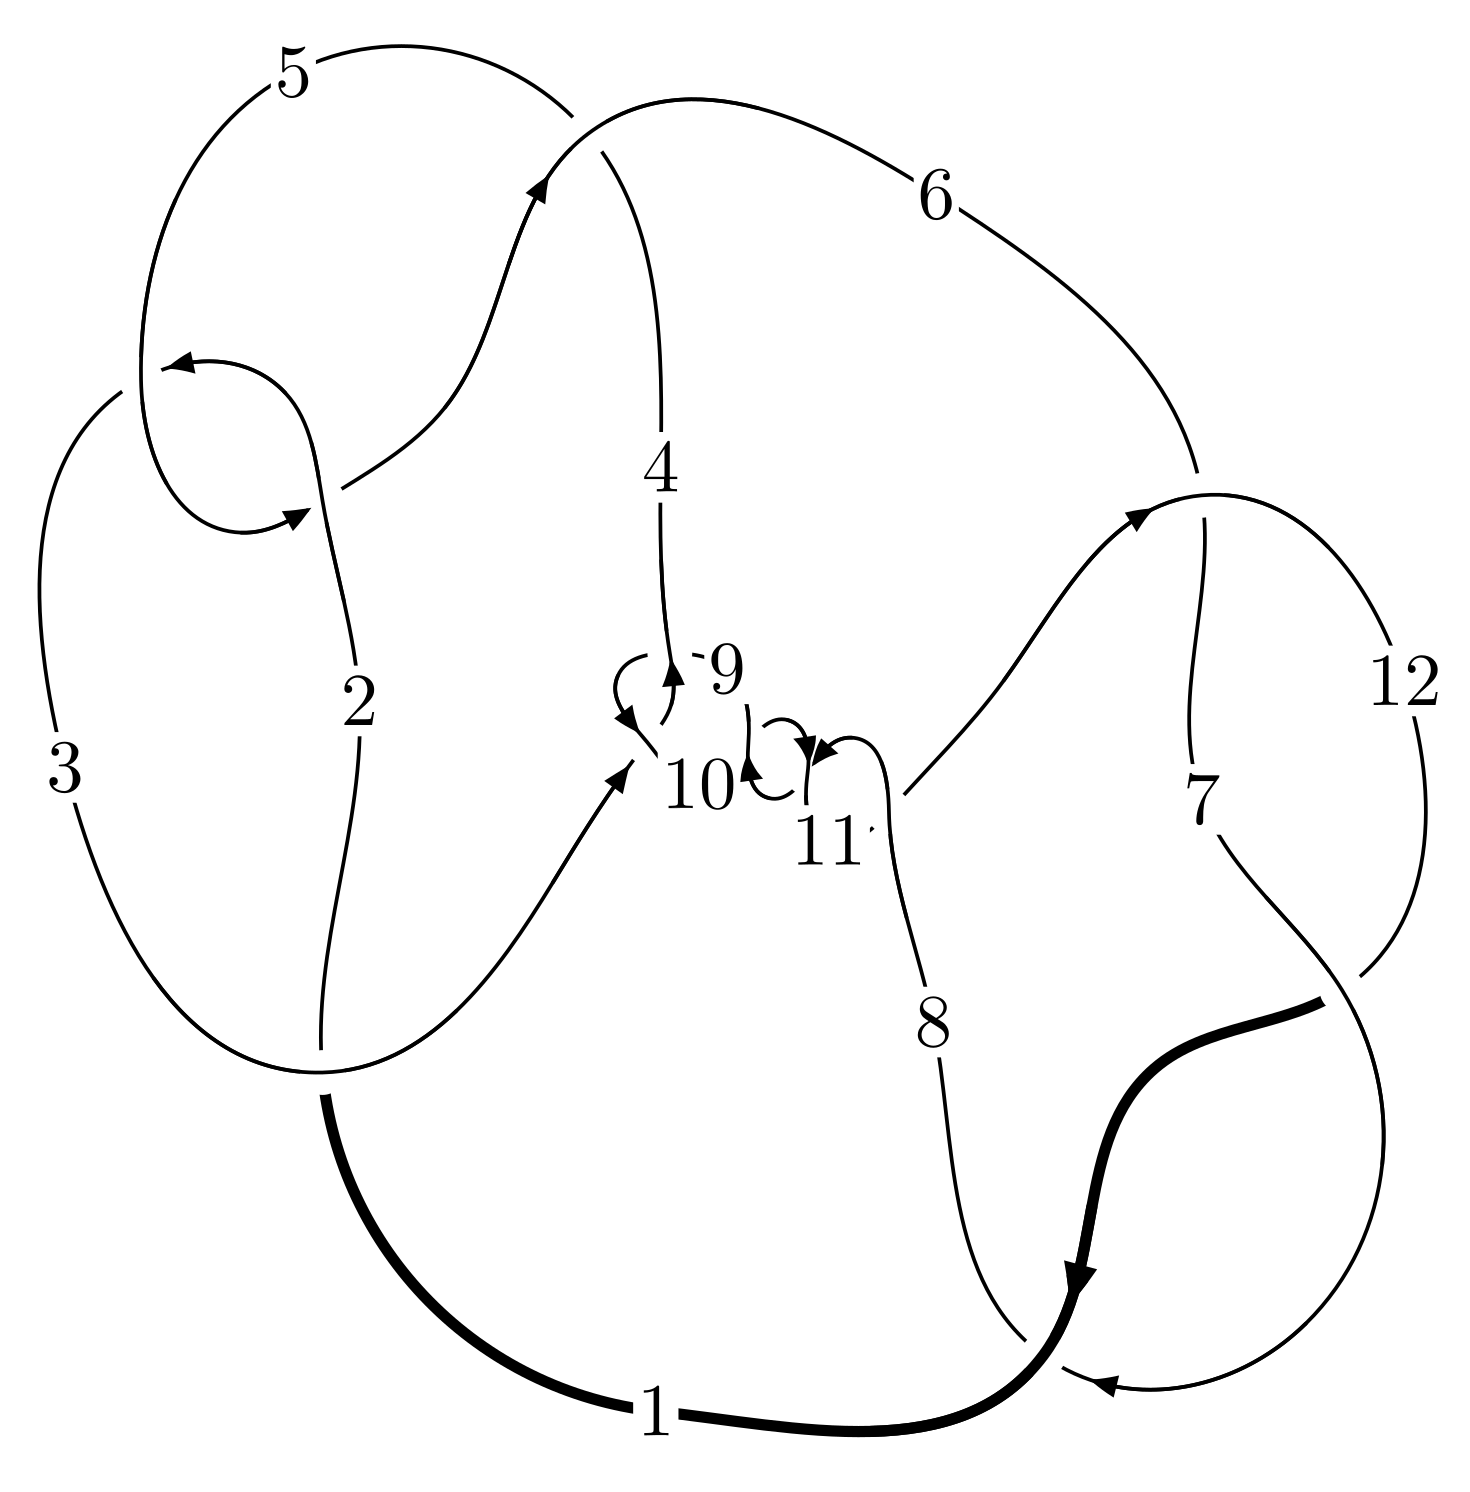
\includegraphics[width=112pt]{../../../GIT/diagram.site/Diagrams/png/997_12a_0196.png}\\
\ \ \ A knot diagram\footnotemark}&
\allowdisplaybreaks
\textbf{Linearized knot diagam} \\
\cline{2-2}
 &
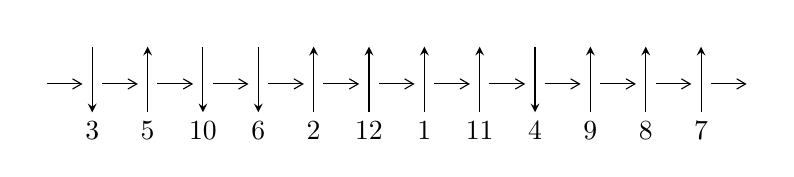
\begin{tikzpicture}[x=20pt, y=17pt]
	% nodes
	\node (C0) at (0, 0) {};
	\node (C1) at (1, 0) {};
	\node (C1U) at (1, +1) {};
	\node (C1D) at (1, -1) {3};

	\node (C2) at (2, 0) {};
	\node (C2U) at (2, +1) {};
	\node (C2D) at (2, -1) {5};

	\node (C3) at (3, 0) {};
	\node (C3U) at (3, +1) {};
	\node (C3D) at (3, -1) {10};

	\node (C4) at (4, 0) {};
	\node (C4U) at (4, +1) {};
	\node (C4D) at (4, -1) {6};

	\node (C5) at (5, 0) {};
	\node (C5U) at (5, +1) {};
	\node (C5D) at (5, -1) {2};

	\node (C6) at (6, 0) {};
	\node (C6U) at (6, +1) {};
	\node (C6D) at (6, -1) {12};

	\node (C7) at (7, 0) {};
	\node (C7U) at (7, +1) {};
	\node (C7D) at (7, -1) {1};

	\node (C8) at (8, 0) {};
	\node (C8U) at (8, +1) {};
	\node (C8D) at (8, -1) {11};

	\node (C9) at (9, 0) {};
	\node (C9U) at (9, +1) {};
	\node (C9D) at (9, -1) {4};

	\node (C10) at (10, 0) {};
	\node (C10U) at (10, +1) {};
	\node (C10D) at (10, -1) {9};

	\node (C11) at (11, 0) {};
	\node (C11U) at (11, +1) {};
	\node (C11D) at (11, -1) {8};

	\node (C12) at (12, 0) {};
	\node (C12U) at (12, +1) {};
	\node (C12D) at (12, -1) {7};
	\node (C13) at (13, 0) {};

	% arrows
	\draw[->,>={angle 60}]
	(C0) edge (C1) (C1) edge (C2) (C2) edge (C3) (C3) edge (C4) (C4) edge (C5) (C5) edge (C6) (C6) edge (C7) (C7) edge (C8) (C8) edge (C9) (C9) edge (C10) (C10) edge (C11) (C11) edge (C12) (C12) edge (C13) ;	\draw[->,>=stealth]
	(C1U) edge (C1D) (C2D) edge (C2U) (C3U) edge (C3D) (C4U) edge (C4D) (C5D) edge (C5U) (C6D) edge (C6U) (C7D) edge (C7U) (C8D) edge (C8U) (C9U) edge (C9D) (C10D) edge (C10U) (C11D) edge (C11U) (C12D) edge (C12U) ;
	\end{tikzpicture} \\
\hhline{~~} \\& 
\textbf{Solving Sequence} \\ \cline{2-2} 
 &
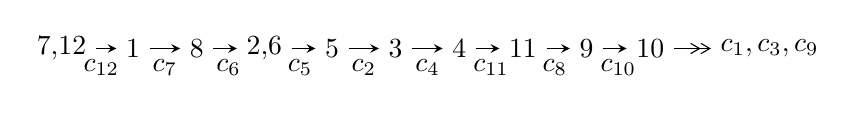
\begin{tikzpicture}[x=23pt, y=7pt]
	% node
	\node (A0) at (-1/8, 0) {7,12};
	\node (A1) at (1, 0) {1};
	\node (A2) at (2, 0) {8};
	\node (A3) at (49/16, 0) {2,6};
	\node (A4) at (33/8, 0) {5};
	\node (A5) at (41/8, 0) {3};
	\node (A6) at (49/8, 0) {4};
	\node (A7) at (57/8, 0) {11};
	\node (A8) at (65/8, 0) {9};
	\node (A9) at (73/8, 0) {10};
	\node (C1) at (1/2, -1) {$c_{12}$};
	\node (C2) at (3/2, -1) {$c_{7}$};
	\node (C3) at (5/2, -1) {$c_{6}$};
	\node (C4) at (29/8, -1) {$c_{5}$};
	\node (C5) at (37/8, -1) {$c_{2}$};
	\node (C6) at (45/8, -1) {$c_{4}$};
	\node (C7) at (53/8, -1) {$c_{11}$};
	\node (C8) at (61/8, -1) {$c_{8}$};
	\node (C9) at (69/8, -1) {$c_{10}$};
	\node (A10) at (11, 0) {$c_{1},c_{3},c_{9}$};

	% edge
	\draw[->,>=stealth]	
	(A0) edge (A1) (A1) edge (A2) (A2) edge (A3) (A3) edge (A4) (A4) edge (A5) (A5) edge (A6) (A6) edge (A7) (A7) edge (A8) (A8) edge (A9) ;
	\draw[->>,>={angle 60}]	
	(A9) edge (A10);
\end{tikzpicture} \\ 

\end{tabular} \\

\footnotetext{
The image of knot diagram is generated by the software ``\textbf{Draw programme}" developed by Andrew Bartholomew(\url{http://www.layer8.co.uk/maths/draw/index.htm\#Running-draw}), where we modified some parts for our purpose(\url{https://github.com/CATsTAILs/LinksPainter}).
}\phantom \\ \newline 
\centering \textbf{Ideals for irreducible components\footnotemark of $X_{\text{par}}$} 
 
\begin{align*}
I^u_{1}&=\langle 
u^{25}-9 u^{23}+\cdots+b+u,\;- u^{64}-2 u^{63}+\cdots+2 a-3,\;u^{65}+3 u^{64}+\cdots+2 u-1\rangle \\
I^u_{2}&=\langle 
b+1,\;a^2- a+1,\;u-1\rangle \\
\\
\end{align*}
\raggedright * 2 irreducible components of $\dim_{\mathbb{C}}=0$, with total 67 representations.\\
\footnotetext{All coefficients of polynomials are rational numbers. But the coefficients are sometimes approximated in decimal forms when there is not enough margin.}
\newpage
\renewcommand{\arraystretch}{1}
\centering \section*{I. $I^u_{1}= \langle u^{25}-9 u^{23}+\cdots+b+u,\;- u^{64}-2 u^{63}+\cdots+2 a-3,\;u^{65}+3 u^{64}+\cdots+2 u-1 \rangle$}
\flushleft \textbf{(i) Arc colorings}\\
\begin{tabular}{m{7pt} m{180pt} m{7pt} m{180pt} }
\flushright $a_{7}=$&$\begin{pmatrix}0\\u\end{pmatrix}$ \\
\flushright $a_{12}=$&$\begin{pmatrix}1\\0\end{pmatrix}$ \\
\flushright $a_{1}=$&$\begin{pmatrix}1\\- u^2\end{pmatrix}$ \\
\flushright $a_{8}=$&$\begin{pmatrix}u\\- u^3+u\end{pmatrix}$ \\
\flushright $a_{2}=$&$\begin{pmatrix}\frac{1}{2} u^{64}+u^{63}+\cdots-\frac{9}{2} u+\frac{3}{2}\\- u^{25}+9 u^{23}+\cdots+4 u^2- u\end{pmatrix}$ \\
\flushright $a_{6}=$&$\begin{pmatrix}- u\\u\end{pmatrix}$ \\
\flushright $a_{5}=$&$\begin{pmatrix}-4 u^{64}-7 u^{63}+\cdots-13 u+3\\\frac{1}{2} u^{64}+u^{63}+\cdots+\frac{5}{2} u-\frac{1}{2}\end{pmatrix}$ \\
\flushright $a_{3}=$&$\begin{pmatrix}-\frac{1}{2} u^{64}- u^{63}+\cdots+\frac{1}{2} u+\frac{3}{2}\\5 u^{64}+9 u^{63}+\cdots+11 u-4\end{pmatrix}$ \\
\flushright $a_{4}=$&$\begin{pmatrix}-\frac{19}{2} u^{64}-17 u^{63}+\cdots-\frac{51}{2} u+\frac{15}{2}\\6 u^{64}+11 u^{63}+\cdots+15 u-5\end{pmatrix}$ \\
\flushright $a_{11}=$&$\begin{pmatrix}- u^4+u^2+1\\u^6-2 u^4+u^2\end{pmatrix}$ \\
\flushright $a_{9}=$&$\begin{pmatrix}u^7-2 u^5+2 u\\- u^9+3 u^7-3 u^5+u\end{pmatrix}$ \\
\flushright $a_{10}=$&$\begin{pmatrix}- u^{10}+3 u^8-2 u^6-3 u^4+3 u^2+1\\u^{12}-4 u^{10}+6 u^8-2 u^6-3 u^4+2 u^2\end{pmatrix}$\\&\end{tabular}
\flushleft \textbf{(ii) Obstruction class $= -1$}\\~\\
\flushleft \textbf{(iii) Cusp Shapes $= -23 u^{64}-35 u^{63}+\cdots-75 u+24$}\\~\\
\newpage\renewcommand{\arraystretch}{1}
\flushleft \textbf{(iv) u-Polynomials at the component}\newline \\
\begin{tabular}{m{50pt}|m{274pt}}
Crossings & \hspace{64pt}u-Polynomials at each crossing \\
\hline $$\begin{aligned}c_{1},c_{4}\end{aligned}$$&$\begin{aligned}
&u^{65}+24 u^{64}+\cdots+7 u-1
\end{aligned}$\\
\hline $$\begin{aligned}c_{2},c_{5}\end{aligned}$$&$\begin{aligned}
&u^{65}+2 u^{64}+\cdots- u+1
\end{aligned}$\\
\hline $$\begin{aligned}c_{3},c_{9}\end{aligned}$$&$\begin{aligned}
&u^{65}- u^{64}+\cdots-4 u-4
\end{aligned}$\\
\hline $$\begin{aligned}c_{6},c_{7},c_{12}\end{aligned}$$&$\begin{aligned}
&u^{65}+3 u^{64}+\cdots+2 u-1
\end{aligned}$\\
\hline $$\begin{aligned}c_{8},c_{10},c_{11}\end{aligned}$$&$\begin{aligned}
&u^{65}-15 u^{64}+\cdots-152 u+16
\end{aligned}$\\
\hline
\end{tabular}\\~\\
\newpage\renewcommand{\arraystretch}{1}
\flushleft \textbf{(v) Riley Polynomials at the component}\newline \\
\begin{tabular}{m{50pt}|m{274pt}}
Crossings & \hspace{64pt}Riley Polynomials at each crossing \\
\hline $$\begin{aligned}c_{1},c_{4}\end{aligned}$$&$\begin{aligned}
&y^{65}+36 y^{64}+\cdots+127 y-1
\end{aligned}$\\
\hline $$\begin{aligned}c_{2},c_{5}\end{aligned}$$&$\begin{aligned}
&y^{65}+24 y^{64}+\cdots+7 y-1
\end{aligned}$\\
\hline $$\begin{aligned}c_{3},c_{9}\end{aligned}$$&$\begin{aligned}
&y^{65}+15 y^{64}+\cdots-152 y-16
\end{aligned}$\\
\hline $$\begin{aligned}c_{6},c_{7},c_{12}\end{aligned}$$&$\begin{aligned}
&y^{65}-51 y^{64}+\cdots-22 y-1
\end{aligned}$\\
\hline $$\begin{aligned}c_{8},c_{10},c_{11}\end{aligned}$$&$\begin{aligned}
&y^{65}+67 y^{64}+\cdots-1760 y-256
\end{aligned}$\\
\hline
\end{tabular}\\~\\
\newpage\flushleft \textbf{(vi) Complex Volumes and Cusp Shapes}
$$\begin{array}{c|c|c}  
\text{Solutions to }I^u_{1}& \I (\text{vol} + \sqrt{-1}CS) & \text{Cusp shape}\\
 \hline 
\begin{aligned}
u &= \phantom{-}0.830964 + 0.370556 I \\
a &= \phantom{-}0.414128 + 1.222280 I \\
b &= -0.659634 - 0.034107 I\end{aligned}
 & \phantom{-}2.82432 - 2.82669 I & \phantom{-}9.20461 + 4.33058 I \\ \hline\begin{aligned}
u &= \phantom{-}0.830964 - 0.370556 I \\
a &= \phantom{-}0.414128 - 1.222280 I \\
b &= -0.659634 + 0.034107 I\end{aligned}
 & \phantom{-}2.82432 + 2.82669 I & \phantom{-}9.20461 - 4.33058 I \\ \hline\begin{aligned}
u &= \phantom{-}0.066558 + 0.901955 I \\
a &= \phantom{-}0.06137 + 1.43251 I \\
b &= -1.28652 - 0.78803 I\end{aligned}
 & -6.76619 + 10.19040 I & \phantom{-0.000000 } 0. - 7.34564 I \\ \hline\begin{aligned}
u &= \phantom{-}0.066558 - 0.901955 I \\
a &= \phantom{-}0.06137 - 1.43251 I \\
b &= -1.28652 + 0.78803 I\end{aligned}
 & -6.76619 - 10.19040 I & \phantom{-0.000000 -}0. + 7.34564 I \\ \hline\begin{aligned}
u &= \phantom{-}0.024152 + 0.893253 I \\
a &= -0.241320 + 0.052855 I \\
b &= \phantom{-}1.52166 - 0.03451 I\end{aligned}
 & -11.12980 + 3.22994 I & -3.82673 - 2.58821 I \\ \hline\begin{aligned}
u &= \phantom{-}0.024152 - 0.893253 I \\
a &= -0.241320 - 0.052855 I \\
b &= \phantom{-}1.52166 + 0.03451 I\end{aligned}
 & -11.12980 - 3.22994 I & -3.82673 + 2.58821 I \\ \hline\begin{aligned}
u &= \phantom{-}0.062913 + 0.882423 I \\
a &= \phantom{-}0.600816 + 0.907451 I \\
b &= -0.0566985 + 0.0369613 I\end{aligned}
 & -5.21752 + 4.69393 I & \phantom{-}2.36653 - 2.83625 I \\ \hline\begin{aligned}
u &= \phantom{-}0.062913 - 0.882423 I \\
a &= \phantom{-}0.600816 - 0.907451 I \\
b &= -0.0566985 - 0.0369613 I\end{aligned}
 & -5.21752 - 4.69393 I & \phantom{-}2.36653 + 2.83625 I \\ \hline\begin{aligned}
u &= \phantom{-}1.11897\phantom{ +0.000000I} \\
a &= \phantom{-}0.950189\phantom{ +0.000000I} \\
b &= -1.18495\phantom{ +0.000000I}\end{aligned}
 & \phantom{-}2.10269\phantom{ +0.000000I} & \phantom{-0.000000 } 0 \\ \hline\begin{aligned}
u &= -0.016371 + 0.867847 I \\
a &= \phantom{-}0.03955 - 1.52936 I \\
b &= -1.27847 + 0.81240 I\end{aligned}
 & -7.11500 - 3.79480 I & -0.49729 + 2.45032 I\\
 \hline 
 \end{array}$$\newpage$$\begin{array}{c|c|c}  
\text{Solutions to }I^u_{1}& \I (\text{vol} + \sqrt{-1}CS) & \text{Cusp shape}\\
 \hline 
\begin{aligned}
u &= -0.016371 - 0.867847 I \\
a &= \phantom{-}0.03955 + 1.52936 I \\
b &= -1.27847 - 0.81240 I\end{aligned}
 & -7.11500 + 3.79480 I & -0.49729 - 2.45032 I \\ \hline\begin{aligned}
u &= \phantom{-}1.114100 + 0.234415 I \\
a &= \phantom{-}1.30619 - 0.76462 I \\
b &= -1.51455 + 0.07170 I\end{aligned}
 & -0.070748 + 1.002540 I & \phantom{-0.000000 } 0 \\ \hline\begin{aligned}
u &= \phantom{-}1.114100 - 0.234415 I \\
a &= \phantom{-}1.30619 + 0.76462 I \\
b &= -1.51455 - 0.07170 I\end{aligned}
 & -0.070748 - 1.002540 I & \phantom{-0.000000 } 0 \\ \hline\begin{aligned}
u &= \phantom{-}0.005459 + 0.854340 I \\
a &= \phantom{-}0.622687 - 0.842608 I \\
b &= -0.0319577 - 0.0652390 I\end{aligned}
 & -5.46649 + 1.55705 I & \phantom{-}1.83939 - 2.39316 I \\ \hline\begin{aligned}
u &= \phantom{-}0.005459 - 0.854340 I \\
a &= \phantom{-}0.622687 + 0.842608 I \\
b &= -0.0319577 + 0.0652390 I\end{aligned}
 & -5.46649 - 1.55705 I & \phantom{-}1.83939 + 2.39316 I \\ \hline\begin{aligned}
u &= \phantom{-}0.715576 + 0.377441 I \\
a &= -0.083470 - 0.122092 I \\
b &= -1.096020 - 0.383591 I\end{aligned}
 & \phantom{-}3.10104 + 2.22312 I & \phantom{-}10.61157 - 3.44892 I \\ \hline\begin{aligned}
u &= \phantom{-}0.715576 - 0.377441 I \\
a &= -0.083470 + 0.122092 I \\
b &= -1.096020 + 0.383591 I\end{aligned}
 & \phantom{-}3.10104 - 2.22312 I & \phantom{-}10.61157 + 3.44892 I \\ \hline\begin{aligned}
u &= -1.201100 + 0.088561 I \\
a &= \phantom{-}0.660258 - 1.069540 I \\
b &= -0.986878 + 0.212897 I\end{aligned}
 & \phantom{-}2.56341 + 1.29431 I & \phantom{-0.000000 } 0 \\ \hline\begin{aligned}
u &= -1.201100 - 0.088561 I \\
a &= \phantom{-}0.660258 + 1.069540 I \\
b &= -0.986878 - 0.212897 I\end{aligned}
 & \phantom{-}2.56341 - 1.29431 I & \phantom{-0.000000 } 0 \\ \hline\begin{aligned}
u &= \phantom{-}1.264370 + 0.105797 I \\
a &= -1.59167 + 2.24205 I \\
b &= \phantom{-}2.07417 - 2.88479 I\end{aligned}
 & \phantom{-}4.34245 - 0.22990 I & \phantom{-0.000000 } 0\\
 \hline 
 \end{array}$$\newpage$$\begin{array}{c|c|c}  
\text{Solutions to }I^u_{1}& \I (\text{vol} + \sqrt{-1}CS) & \text{Cusp shape}\\
 \hline 
\begin{aligned}
u &= \phantom{-}1.264370 - 0.105797 I \\
a &= -1.59167 - 2.24205 I \\
b &= \phantom{-}2.07417 + 2.88479 I\end{aligned}
 & \phantom{-}4.34245 + 0.22990 I & \phantom{-0.000000 } 0 \\ \hline\begin{aligned}
u &= -1.253070 + 0.208336 I \\
a &= \phantom{-}1.03231 + 1.06068 I \\
b &= -1.314840 - 0.300085 I\end{aligned}
 & \phantom{-}1.07506 - 4.90470 I & \phantom{-0.000000 } 0 \\ \hline\begin{aligned}
u &= -1.253070 - 0.208336 I \\
a &= \phantom{-}1.03231 - 1.06068 I \\
b &= -1.314840 + 0.300085 I\end{aligned}
 & \phantom{-}1.07506 + 4.90470 I & \phantom{-0.000000 } 0 \\ \hline\begin{aligned}
u &= \phantom{-}0.296526 + 0.660870 I \\
a &= -0.417175 + 0.983556 I \\
b &= -1.162320 - 0.683557 I\end{aligned}
 & \phantom{-}1.24443 + 6.73457 I & \phantom{-}4.49555 - 9.38933 I \\ \hline\begin{aligned}
u &= \phantom{-}0.296526 - 0.660870 I \\
a &= -0.417175 - 0.983556 I \\
b &= -1.162320 + 0.683557 I\end{aligned}
 & \phantom{-}1.24443 - 6.73457 I & \phantom{-}4.49555 + 9.38933 I \\ \hline\begin{aligned}
u &= \phantom{-}1.271700 + 0.149643 I \\
a &= -3.61249 - 0.52455 I \\
b &= \phantom{-}4.21319 + 1.18292 I\end{aligned}
 & \phantom{-}3.83870 + 4.96968 I & \phantom{-0.000000 } 0 \\ \hline\begin{aligned}
u &= \phantom{-}1.271700 - 0.149643 I \\
a &= -3.61249 + 0.52455 I \\
b &= \phantom{-}4.21319 - 1.18292 I\end{aligned}
 & \phantom{-}3.83870 - 4.96968 I & \phantom{-0.000000 } 0 \\ \hline\begin{aligned}
u &= -1.280910 + 0.122024 I \\
a &= \phantom{-}0.841025 + 0.030121 I \\
b &= -1.319450 + 0.068717 I\end{aligned}
 & \phantom{-}4.74156 - 2.53764 I & \phantom{-0.000000 } 0 \\ \hline\begin{aligned}
u &= -1.280910 - 0.122024 I \\
a &= \phantom{-}0.841025 - 0.030121 I \\
b &= -1.319450 - 0.068717 I\end{aligned}
 & \phantom{-}4.74156 + 2.53764 I & \phantom{-0.000000 } 0 \\ \hline\begin{aligned}
u &= \phantom{-}1.217380 + 0.430410 I \\
a &= \phantom{-}0.645359 + 0.037607 I \\
b &= -1.339890 - 0.221192 I\end{aligned}
 & -1.65945 + 0.00019 I & \phantom{-0.000000 } 0\\
 \hline 
 \end{array}$$\newpage$$\begin{array}{c|c|c}  
\text{Solutions to }I^u_{1}& \I (\text{vol} + \sqrt{-1}CS) & \text{Cusp shape}\\
 \hline 
\begin{aligned}
u &= \phantom{-}1.217380 - 0.430410 I \\
a &= \phantom{-}0.645359 - 0.037607 I \\
b &= -1.339890 + 0.221192 I\end{aligned}
 & -1.65945 - 0.00019 I & \phantom{-0.000000 } 0 \\ \hline\begin{aligned}
u &= \phantom{-}1.221140 + 0.453912 I \\
a &= \phantom{-}0.546680 + 1.232540 I \\
b &= -0.731588 - 0.300425 I\end{aligned}
 & -3.20943 - 5.35553 I & \phantom{-0.000000 } 0 \\ \hline\begin{aligned}
u &= \phantom{-}1.221140 - 0.453912 I \\
a &= \phantom{-}0.546680 - 1.232540 I \\
b &= -0.731588 + 0.300425 I\end{aligned}
 & -3.20943 + 5.35553 I & \phantom{-0.000000 } 0 \\ \hline\begin{aligned}
u &= \phantom{-}0.331431 + 0.600598 I \\
a &= \phantom{-}0.71215 + 1.26973 I \\
b &= -0.283162 + 0.112072 I\end{aligned}
 & \phantom{-}1.96106 + 1.49753 I & \phantom{-}6.66169 - 4.12095 I \\ \hline\begin{aligned}
u &= \phantom{-}0.331431 - 0.600598 I \\
a &= \phantom{-}0.71215 - 1.26973 I \\
b &= -0.283162 - 0.112072 I\end{aligned}
 & \phantom{-}1.96106 - 1.49753 I & \phantom{-}6.66169 + 4.12095 I \\ \hline\begin{aligned}
u &= -1.261550 + 0.406598 I \\
a &= \phantom{-}0.567428 - 1.227950 I \\
b &= -0.768468 + 0.314906 I\end{aligned}
 & -3.25565 - 0.77125 I & \phantom{-0.000000 } 0 \\ \hline\begin{aligned}
u &= -1.261550 - 0.406598 I \\
a &= \phantom{-}0.567428 + 1.227950 I \\
b &= -0.768468 - 0.314906 I\end{aligned}
 & -3.25565 + 0.77125 I & \phantom{-0.000000 } 0 \\ \hline\begin{aligned}
u &= \phantom{-}1.270390 + 0.393882 I \\
a &= -0.371976 + 0.875631 I \\
b &= \phantom{-}0.81144 - 1.43667 I\end{aligned}
 & -1.53986 + 2.92050 I & \phantom{-0.000000 } 0 \\ \hline\begin{aligned}
u &= \phantom{-}1.270390 - 0.393882 I \\
a &= -0.371976 - 0.875631 I \\
b &= \phantom{-}0.81144 + 1.43667 I\end{aligned}
 & -1.53986 - 2.92050 I & \phantom{-0.000000 } 0 \\ \hline\begin{aligned}
u &= \phantom{-}1.259520 + 0.431707 I \\
a &= \phantom{-}1.19388 - 1.33090 I \\
b &= -1.47420 + 0.52784 I\end{aligned}
 & -7.30459 + 1.50541 I & \phantom{-0.000000 } 0\\
 \hline 
 \end{array}$$\newpage$$\begin{array}{c|c|c}  
\text{Solutions to }I^u_{1}& \I (\text{vol} + \sqrt{-1}CS) & \text{Cusp shape}\\
 \hline 
\begin{aligned}
u &= \phantom{-}1.259520 - 0.431707 I \\
a &= \phantom{-}1.19388 + 1.33090 I \\
b &= -1.47420 - 0.52784 I\end{aligned}
 & -7.30459 - 1.50541 I & \phantom{-0.000000 } 0 \\ \hline\begin{aligned}
u &= -1.279100 + 0.393239 I \\
a &= \phantom{-}0.701587 - 0.036472 I \\
b &= -1.358830 + 0.193709 I\end{aligned}
 & -1.47317 - 6.03292 I & \phantom{-0.000000 } 0 \\ \hline\begin{aligned}
u &= -1.279100 - 0.393239 I \\
a &= \phantom{-}0.701587 + 0.036472 I \\
b &= -1.358830 - 0.193709 I\end{aligned}
 & -1.47317 + 6.03292 I & \phantom{-0.000000 } 0 \\ \hline\begin{aligned}
u &= \phantom{-}1.288150 + 0.402371 I \\
a &= -2.76510 + 0.75793 I \\
b &= \phantom{-}3.46338 - 0.15706 I\end{aligned}
 & -3.05519 + 8.34787 I & \phantom{-0.000000 } 0 \\ \hline\begin{aligned}
u &= \phantom{-}1.288150 - 0.402371 I \\
a &= -2.76510 - 0.75793 I \\
b &= \phantom{-}3.46338 + 0.15706 I\end{aligned}
 & -3.05519 - 8.34787 I & \phantom{-0.000000 } 0 \\ \hline\begin{aligned}
u &= -1.297920 + 0.419236 I \\
a &= \phantom{-}1.14982 + 1.32131 I \\
b &= -1.43370 - 0.52696 I\end{aligned}
 & -7.01228 - 7.92581 I & \phantom{-0.000000 } 0 \\ \hline\begin{aligned}
u &= -1.297920 - 0.419236 I \\
a &= \phantom{-}1.14982 - 1.32131 I \\
b &= -1.43370 + 0.52696 I\end{aligned}
 & -7.01228 + 7.92581 I & \phantom{-0.000000 } 0 \\ \hline\begin{aligned}
u &= -1.355680 + 0.197509 I \\
a &= -1.18478 - 1.33241 I \\
b &= \phantom{-}1.66192 + 1.92791 I\end{aligned}
 & \phantom{-}7.25490 - 4.25204 I & \phantom{-0.000000 } 0 \\ \hline\begin{aligned}
u &= -1.355680 - 0.197509 I \\
a &= -1.18478 + 1.33241 I \\
b &= \phantom{-}1.66192 - 1.92791 I\end{aligned}
 & \phantom{-}7.25490 + 4.25204 I & \phantom{-0.000000 } 0 \\ \hline\begin{aligned}
u &= -1.358940 + 0.225362 I \\
a &= -2.94873 + 0.05360 I \\
b &= \phantom{-}3.57045 - 0.66704 I\end{aligned}
 & \phantom{-}6.47155 - 9.82570 I & \phantom{-0.000000 } 0\\
 \hline 
 \end{array}$$\newpage$$\begin{array}{c|c|c}  
\text{Solutions to }I^u_{1}& \I (\text{vol} + \sqrt{-1}CS) & \text{Cusp shape}\\
 \hline 
\begin{aligned}
u &= -1.358940 - 0.225362 I \\
a &= -2.94873 - 0.05360 I \\
b &= \phantom{-}3.57045 + 0.66704 I\end{aligned}
 & \phantom{-}6.47155 + 9.82570 I & \phantom{-0.000000 } 0 \\ \hline\begin{aligned}
u &= -1.378690 + 0.015478 I \\
a &= -2.40374 + 1.10451 I \\
b &= \phantom{-}2.94698 - 1.72078 I\end{aligned}
 & \phantom{-}9.54691 - 2.80083 I & \phantom{-0.000000 } 0 \\ \hline\begin{aligned}
u &= -1.378690 - 0.015478 I \\
a &= -2.40374 - 1.10451 I \\
b &= \phantom{-}2.94698 + 1.72078 I\end{aligned}
 & \phantom{-}9.54691 + 2.80083 I & \phantom{-0.000000 } 0 \\ \hline\begin{aligned}
u &= -1.322040 + 0.404776 I \\
a &= -0.523462 - 0.791434 I \\
b &= \phantom{-}0.97175 + 1.35042 I\end{aligned}
 & -0.88717 - 9.30751 I & \phantom{-0.000000 } 0 \\ \hline\begin{aligned}
u &= -1.322040 - 0.404776 I \\
a &= -0.523462 + 0.791434 I \\
b &= \phantom{-}0.97175 - 1.35042 I\end{aligned}
 & -0.88717 + 9.30751 I & \phantom{-0.000000 } 0 \\ \hline\begin{aligned}
u &= -1.328270 + 0.415651 I \\
a &= -2.64876 - 0.66443 I \\
b &= \phantom{-}3.34028 + 0.07943 I\end{aligned}
 & -2.4034 - 14.9064 I & \phantom{-0.000000 } 0 \\ \hline\begin{aligned}
u &= -1.328270 - 0.415651 I \\
a &= -2.64876 + 0.66443 I \\
b &= \phantom{-}3.34028 - 0.07943 I\end{aligned}
 & -2.4034 + 14.9064 I & \phantom{-0.000000 } 0 \\ \hline\begin{aligned}
u &= \phantom{-}0.093193 + 0.588157 I \\
a &= \phantom{-}0.617551 + 0.336841 I \\
b &= \phantom{-}0.947496 - 0.243938 I\end{aligned}
 & -3.01176 + 2.07036 I & -3.85437 - 4.88526 I \\ \hline\begin{aligned}
u &= \phantom{-}0.093193 - 0.588157 I \\
a &= \phantom{-}0.617551 - 0.336841 I \\
b &= \phantom{-}0.947496 + 0.243938 I\end{aligned}
 & -3.01176 - 2.07036 I & -3.85437 + 4.88526 I \\ \hline\begin{aligned}
u &= -0.129828 + 0.412841 I \\
a &= -1.47954 - 1.43101 I \\
b &= -0.988859 + 0.789862 I\end{aligned}
 & -0.41631 - 2.93173 I & -1.44022 + 3.23621 I\\
 \hline 
 \end{array}$$\newpage$$\begin{array}{c|c|c}  
\text{Solutions to }I^u_{1}& \I (\text{vol} + \sqrt{-1}CS) & \text{Cusp shape}\\
 \hline 
\begin{aligned}
u &= -0.129828 - 0.412841 I \\
a &= -1.47954 + 1.43101 I \\
b &= -0.988859 - 0.789862 I\end{aligned}
 & -0.41631 + 2.93173 I & -1.44022 - 3.23621 I \\ \hline\begin{aligned}
u &= \phantom{-}0.225456 + 0.313448 I \\
a &= \phantom{-}0.977902 - 0.161888 I \\
b &= \phantom{-}0.0023464 - 0.1336720 I\end{aligned}
 & \phantom{-}0.265807 + 0.934765 I & \phantom{-}5.23289 - 7.07384 I \\ \hline\begin{aligned}
u &= \phantom{-}0.225456 - 0.313448 I \\
a &= \phantom{-}0.977902 + 0.161888 I \\
b &= \phantom{-}0.0023464 + 0.1336720 I\end{aligned}
 & \phantom{-}0.265807 - 0.934765 I & \phantom{-}5.23289 + 7.07384 I \\ \hline\begin{aligned}
u &= -0.154982 + 0.228760 I \\
a &= \phantom{-}1.60645 - 2.67271 I \\
b &= -0.346535 - 0.504076 I\end{aligned}
 & \phantom{-}0.14978 + 1.56979 I & -1.36396 - 3.31802 I \\ \hline\begin{aligned}
u &= -0.154982 - 0.228760 I \\
a &= \phantom{-}1.60645 + 2.67271 I \\
b &= -0.346535 + 0.504076 I\end{aligned}
 & \phantom{-}0.14978 - 1.56979 I & -1.36396 + 3.31802 I\\
 \hline 
 \end{array}$$\newpage\newpage\renewcommand{\arraystretch}{1}
\centering \section*{II. $I^u_{2}= \langle b+1,\;a^2- a+1,\;u-1 \rangle$}
\flushleft \textbf{(i) Arc colorings}\\
\begin{tabular}{m{7pt} m{180pt} m{7pt} m{180pt} }
\flushright $a_{7}=$&$\begin{pmatrix}0\\1\end{pmatrix}$ \\
\flushright $a_{12}=$&$\begin{pmatrix}1\\0\end{pmatrix}$ \\
\flushright $a_{1}=$&$\begin{pmatrix}1\\-1\end{pmatrix}$ \\
\flushright $a_{8}=$&$\begin{pmatrix}1\\0\end{pmatrix}$ \\
\flushright $a_{2}=$&$\begin{pmatrix}a\\-1\end{pmatrix}$ \\
\flushright $a_{6}=$&$\begin{pmatrix}-1\\1\end{pmatrix}$ \\
\flushright $a_{5}=$&$\begin{pmatrix}0\\a\end{pmatrix}$ \\
\flushright $a_{3}=$&$\begin{pmatrix}a\\0\end{pmatrix}$ \\
\flushright $a_{4}=$&$\begin{pmatrix}a\\0\end{pmatrix}$ \\
\flushright $a_{11}=$&$\begin{pmatrix}1\\0\end{pmatrix}$ \\
\flushright $a_{9}=$&$\begin{pmatrix}1\\0\end{pmatrix}$ \\
\flushright $a_{10}=$&$\begin{pmatrix}1\\0\end{pmatrix}$\\&\end{tabular}
\flushleft \textbf{(ii) Obstruction class $= 1$}\\~\\
\flushleft \textbf{(iii) Cusp Shapes $= 4 a+1$}\\~\\
\newpage\renewcommand{\arraystretch}{1}
\flushleft \textbf{(iv) u-Polynomials at the component}\newline \\
\begin{tabular}{m{50pt}|m{274pt}}
Crossings & \hspace{64pt}u-Polynomials at each crossing \\
\hline $$\begin{aligned}c_{1},c_{4},c_{5}\end{aligned}$$&$\begin{aligned}
&u^2- u+1
\end{aligned}$\\
\hline $$\begin{aligned}c_{2}\end{aligned}$$&$\begin{aligned}
&u^2+u+1
\end{aligned}$\\
\hline $$\begin{aligned}c_{3},c_{8},c_{9}\\c_{10},c_{11}\end{aligned}$$&$\begin{aligned}
&u^2
\end{aligned}$\\
\hline $$\begin{aligned}c_{6},c_{7}\end{aligned}$$&$\begin{aligned}
&(u+1)^2
\end{aligned}$\\
\hline $$\begin{aligned}c_{12}\end{aligned}$$&$\begin{aligned}
&(u-1)^2
\end{aligned}$\\
\hline
\end{tabular}\\~\\
\newpage\renewcommand{\arraystretch}{1}
\flushleft \textbf{(v) Riley Polynomials at the component}\newline \\
\begin{tabular}{m{50pt}|m{274pt}}
Crossings & \hspace{64pt}Riley Polynomials at each crossing \\
\hline $$\begin{aligned}c_{1},c_{2},c_{4}\\c_{5}\end{aligned}$$&$\begin{aligned}
&y^2+y+1
\end{aligned}$\\
\hline $$\begin{aligned}c_{3},c_{8},c_{9}\\c_{10},c_{11}\end{aligned}$$&$\begin{aligned}
&y^2
\end{aligned}$\\
\hline $$\begin{aligned}c_{6},c_{7},c_{12}\end{aligned}$$&$\begin{aligned}
&(y-1)^2
\end{aligned}$\\
\hline
\end{tabular}\\~\\
\newpage\flushleft \textbf{(vi) Complex Volumes and Cusp Shapes}
$$\begin{array}{c|c|c}  
\text{Solutions to }I^u_{2}& \I (\text{vol} + \sqrt{-1}CS) & \text{Cusp shape}\\
 \hline 
\begin{aligned}
u &= \phantom{-}1.00000\phantom{ +0.000000I} \\
a &= \phantom{-}0.500000 + 0.866025 I \\
b &= -1.00000\phantom{ +0.000000I}\end{aligned}
 & \phantom{-}1.64493 - 2.02988 I & \phantom{-}3.00000 + 3.46410 I \\ \hline\begin{aligned}
u &= \phantom{-}1.00000\phantom{ +0.000000I} \\
a &= \phantom{-}0.500000 - 0.866025 I \\
b &= -1.00000\phantom{ +0.000000I}\end{aligned}
 & \phantom{-}1.64493 + 2.02988 I & \phantom{-}3.00000 - 3.46410 I\\
 \hline 
 \end{array}$$\newpage
\newpage\renewcommand{\arraystretch}{1}
\centering \section*{ III. u-Polynomials}
\begin{tabular}{m{50pt}|m{274pt}}
Crossings & \hspace{64pt}u-Polynomials at each crossing \\
\hline $$\begin{aligned}c_{1},c_{4}\end{aligned}$$&$\begin{aligned}
&(u^2- u+1)(u^{65}+24 u^{64}+\cdots+7 u-1)
\end{aligned}$\\
\hline $$\begin{aligned}c_{2}\end{aligned}$$&$\begin{aligned}
&(u^2+u+1)(u^{65}+2 u^{64}+\cdots- u+1)
\end{aligned}$\\
\hline $$\begin{aligned}c_{3},c_{9}\end{aligned}$$&$\begin{aligned}
&u^2(u^{65}- u^{64}+\cdots-4 u-4)
\end{aligned}$\\
\hline $$\begin{aligned}c_{5}\end{aligned}$$&$\begin{aligned}
&(u^2- u+1)(u^{65}+2 u^{64}+\cdots- u+1)
\end{aligned}$\\
\hline $$\begin{aligned}c_{6},c_{7}\end{aligned}$$&$\begin{aligned}
&((u+1)^2)(u^{65}+3 u^{64}+\cdots+2 u-1)
\end{aligned}$\\
\hline $$\begin{aligned}c_{8},c_{10},c_{11}\end{aligned}$$&$\begin{aligned}
&u^2(u^{65}-15 u^{64}+\cdots-152 u+16)
\end{aligned}$\\
\hline $$\begin{aligned}c_{12}\end{aligned}$$&$\begin{aligned}
&((u-1)^2)(u^{65}+3 u^{64}+\cdots+2 u-1)
\end{aligned}$\\
\hline
\end{tabular}\newpage\renewcommand{\arraystretch}{1}
\centering \section*{ IV. Riley Polynomials}
\begin{tabular}{m{50pt}|m{274pt}}
Crossings & \hspace{64pt}Riley Polynomials at each crossing \\
\hline $$\begin{aligned}c_{1},c_{4}\end{aligned}$$&$\begin{aligned}
&(y^2+y+1)(y^{65}+36 y^{64}+\cdots+127 y-1)
\end{aligned}$\\
\hline $$\begin{aligned}c_{2},c_{5}\end{aligned}$$&$\begin{aligned}
&(y^2+y+1)(y^{65}+24 y^{64}+\cdots+7 y-1)
\end{aligned}$\\
\hline $$\begin{aligned}c_{3},c_{9}\end{aligned}$$&$\begin{aligned}
&y^2(y^{65}+15 y^{64}+\cdots-152 y-16)
\end{aligned}$\\
\hline $$\begin{aligned}c_{6},c_{7},c_{12}\end{aligned}$$&$\begin{aligned}
&((y-1)^2)(y^{65}-51 y^{64}+\cdots-22 y-1)
\end{aligned}$\\
\hline $$\begin{aligned}c_{8},c_{10},c_{11}\end{aligned}$$&$\begin{aligned}
&y^2(y^{65}+67 y^{64}+\cdots-1760 y-256)
\end{aligned}$\\
\hline
\end{tabular}
\vskip 2pc
\end{document}